\subsection*{Evaluation}

\begin{itemize}
    \item \textbf{\underline{Programming Languages:}} In order to thoroughly evaluate and understand the different technologies involved, it is useful to distinguish and study various categories under programming languages that are of concern. All the categories below will compare compiled languages such as C/C++ to interpreted languages such as Python/R. 
    
    \begin{itemize}
        \item Speed: Generally in the area of molecular computing or scientific computing in general, speed is of great concern since the simulations should run in a relatively short period of time. Due to this, languages such as C/C++ or MATLAB are often used since they efficiently compute the computations. On the other hand, interpreted code is significantly slower than compiled code in most cases and it truly makes a difference in the scientific computing realm.
        
        \item Portability: Interpreted languages such as Python dominate this particular field because if the user wants to run an application, he or she can execute the script on any platform desired. On the other hand, languages such as C/C++ are specific to the architecture on which it is being run and hence the code has to be compiled using external tools such as \verb|gcc| or \verb|clang|. 
        
        \item Usability: Higher level functionality such as parsing XML files, crawling the web, scanning through files in a filesystem are more involved and harder to write in low-level languages such as C/C++ when compared to interpreted or scripting languages such as Python or R.  In addition, external libraries have to be linked manually, which might be tedious in some cases to run applications using C/C++. On the other hand, this is rarely a problem for Python since libraries can be imported ``on the spot'' and the application can immediately be run.
        
        \item Readability: Generally speaking, Python code tends to fewer lines of code when compared to C/C++ code due to the nature of abstraction and other factors such as syntax and semantics. This is of a significant advantage when developing with very large scientific computing applications since a plethora of script files can be easily understood and examined broadly speaking (when compared to the header and source files for C/C++). 
        
        \item Static vs Dynamic: There has been a lot of research in this area. In most cases, research has shown that static typing produces less bugs when compared to dynamic typing. (This study was performed with Java vs Groovy (will include the citation later)). However, during the development on this project in particular, we rarely encountered issues with the typing and in some cases, dynamic typing was actually helpful with Python since it led to less verbose and concise code.  
    \end{itemize}
    
    \textbf{After considering all the criterion above, the main language that was finally chosen for the computation phase was Python.}
    
    \item \textbf{\underline{Visualization:}} After the appropriate results are computed using the precompiled or interpreted languages, it can be helpful to visualize the results in order to expand and gain more knowledge in the particular area of concern. In relation to this particular project, the following frameworks below was analyzed and throughly evaluated:
    
    
    \begin{itemize}
        \item Matplotlib: As the documentation for the framework proclaims, ``Matplotlib is a Python 2D plotting library which produces publication quality figures in a variety of hardcopy formats and interactive environments across platforms. Matplotlib can be used in Python scripts, the Python and IPython shell, the jupyter notebook, web application servers, and four graphical user interface toolkits.'' This particular library is powerful and offers a lot of features, however one con of the framework is that the library is external to python and has to be installed on the system in order to be used. In other words, if the user wants to run any script which uses the \verb|matplotlib| library, he or she will have to download and integrate the external package with python. Doing so might take a while since the \verb|matplotlib| library also has other dependencies. So even though this solution is rich and powerful, it is not very portable since it assumes that the user has installed the package before running the corresponding script.\newline
        
        % \begin{figure}
        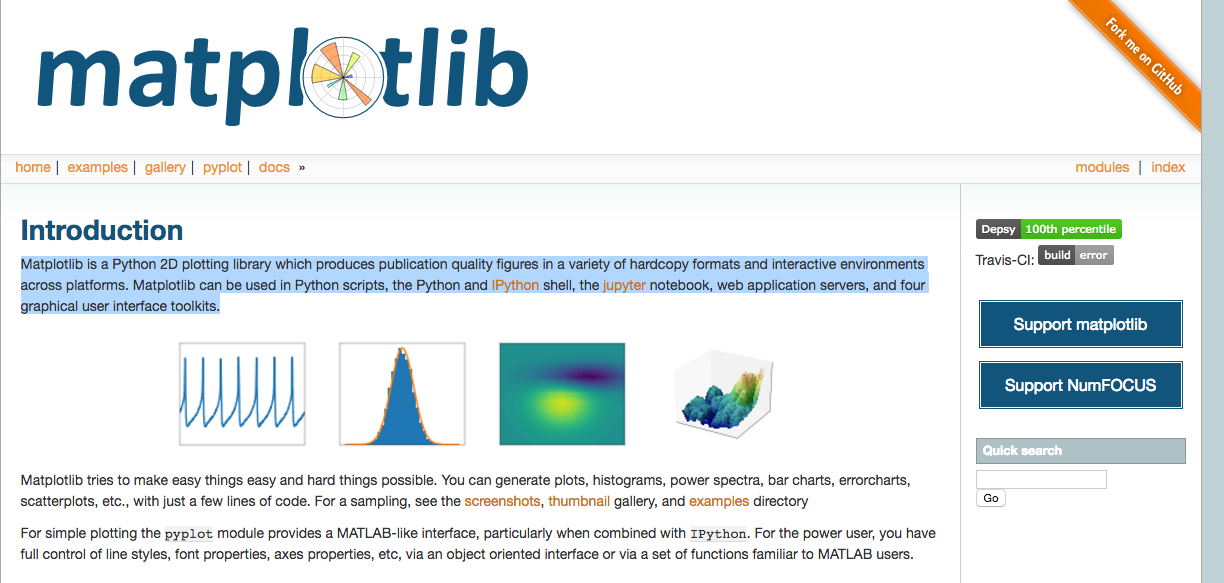
\includegraphics[scale=0.30]{images/matplotlib}\newline
        % \centering
        % \end{figure}
        
        
        \item Bokeh: This particular Python framework is elegant and highly interactive. It provides multiple functions to construct sophisticated graphs and charts, similar to the quality of popular frameworks such as \textit{D3.js}. Even though the library offers a range of useful features, there are a lot of dependencies involved (the documentation clearly highlights all the dependencies: \verb|NumPy, Jinja2, Six,|
        \verb|Requests, Tornado >= 4.0,  PyYaml, DateUtil|). Since this particular framework assumes the installation of the python libraries, it is very difficult for a user to quicky execute and obtain results by merely running the script. \newline
        
        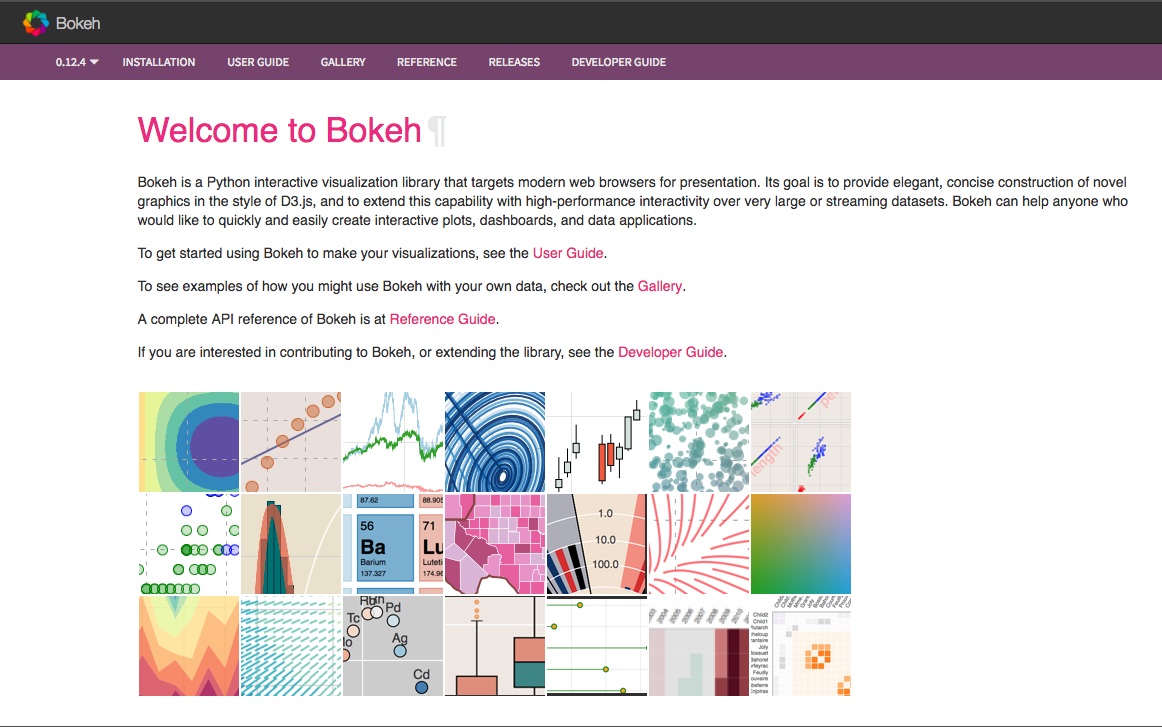
\includegraphics[scale=0.30]{images/bokeh} \newpage
        
        \item Plot.ly: Plot.ly is a highly sophisticated visualization tool which is used by multiple developers from all fields including business analytics and data science. Even though this is a great framework to use, some of the more advanced features have been commercialized and hence not an ``ideal'' solution for the average researcher who is running the scripts for the application. \newline
        
\includegraphics[scale=0.25]{images/plotly}
        
        \item Charts: Charts is a visualization library built entirely out of Javascript. This implies that figures and charts can be easily be developed and displayed by merely opening a web browser. This offers a very portable and a usable solution. In addition, this particular framework is customizable in terms of user's events, and therefore can be advantageous in many situations.\newline \newline
        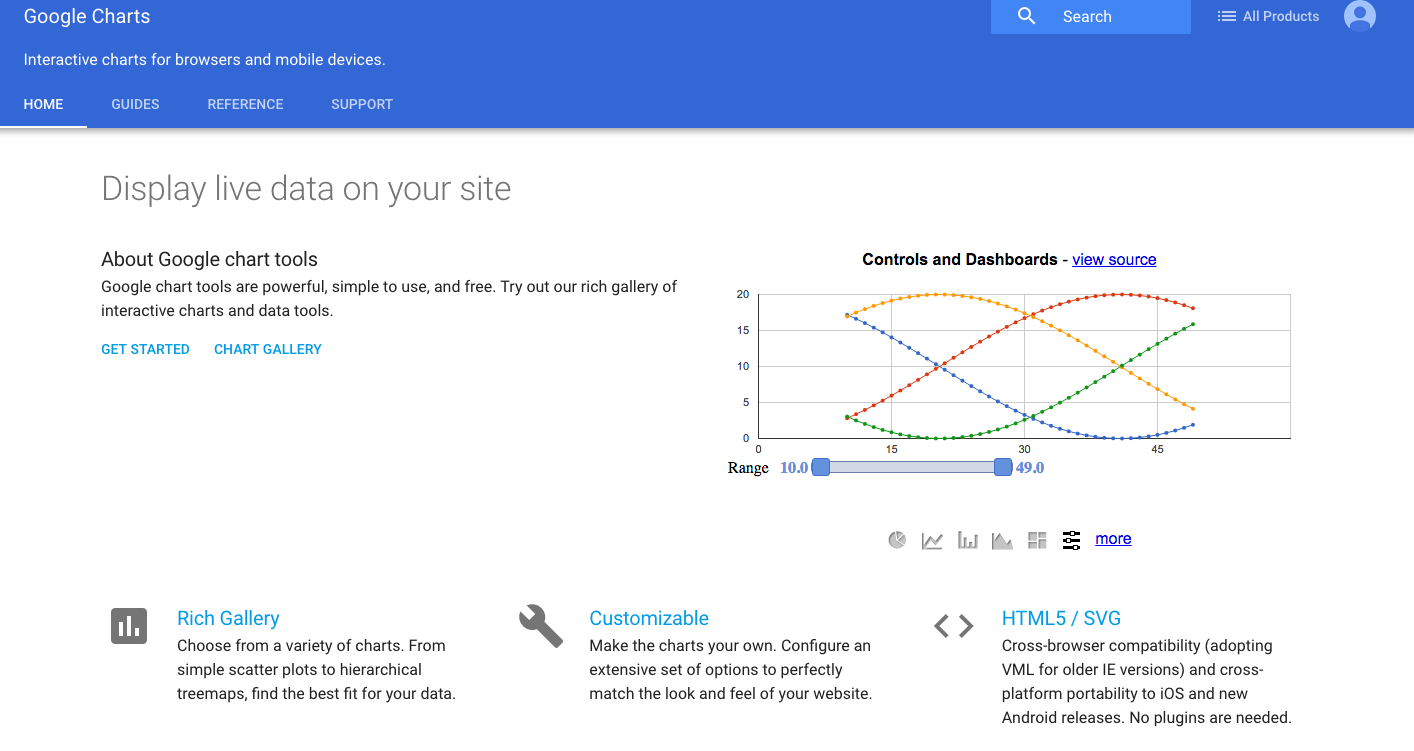
\includegraphics[scale=0.27]{images/charts}
    \end{itemize}
    
    Based on the following criterion, \textit{Charts} was chosen as the visualization platform with the development done in Javascript. The way this is particularly used is that a python script writes the results of the computation phase to a html file containing Javascript code and a call to the Charts library. Doing so offers the best and portable solution to the application that is desired.  
        
\end{itemize}

